\textbf{\underline{OZ 4 - De wet van Ampère en de wet van Biot-Savart - Oefening 2:}}
\vspace{0.5cm}

\begin{minipage}{0.7\textwidth}
    Een circuit bestaat uit twee bogen met straal $R$ en twee rechte stukken op een afstand $2a$ van elkaar. Door het circuit loopt een stroom $I$. Bereken het magneetveld $\vec{B}$ in het punt $P = 0$, gelegen in het vlak van het circuit
    \vspace{1.5cm}
\end{minipage}
\begin{minipage}{0.26\textwidth}
    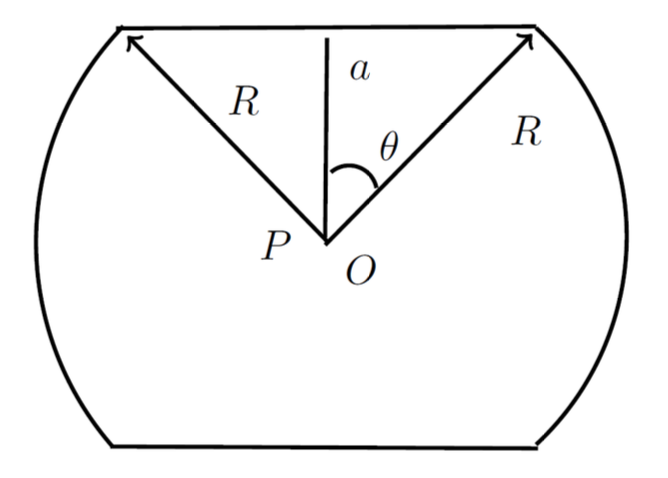
\includegraphics[scale = 0.35]{oz04/resources/Oz4Oef2.png}
\end{minipage}

% \begin{center}
%     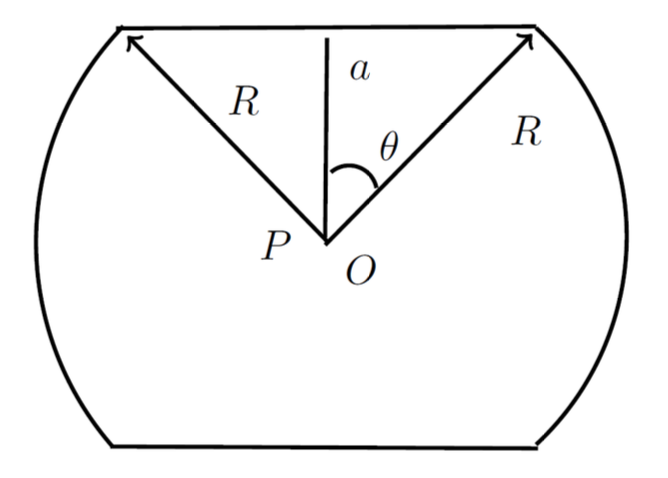
\includegraphics[scale = 0.4]{oz04/resources/Oz4Oef2.png}
% \end{center}
\vspace{-1.5cm}

\begin{description}[labelwidth=1.5cm, leftmargin=!]
    \item[Geg. :]   $R$, $a$, $I$
    \item[Gevr. :]  $\Vec{A}$ ?
    \item[Opl. :]  
    We zullen de vectoriële aanbrenging van de rechte stukken en bogen apart berekenen:
    \begin{itemize}
        \item 
            We integreren over alle infinitesimale magnetische velden geproduceerd door een recht stuk 
            \begin{align*}
                \vec{B}_{|} 
                    &= \int d\Vec{B}_{|} \\
                    &= \frac{\mu_0I}{4\pi}\int\frac{d\ell}{r^2} \sin(\phi) \ (-\hat{k}) \\
                    &= \frac{\mu_0I}{4\pi}\frac{1}{a} \int \sin(\phi) d\phi  \ (-\hat{k}) \\
                    &= \frac{\mu_0I}{2\pi}\frac{1}{a} \int_{\phi}^{\frac{\pi}{2}} \sin(\phi) d\phi  \ (-\hat{k}) \\
                    &= \frac{\mu_0I}{2\pi}\frac{1}{a} \cos(\phi) \ (-\hat{k}) \\
                    &= \frac{\mu_0I}{2\pi}\frac{1}{a} \frac{\sqrt{R^2-a^2}}{R} \ (-\hat{k}) \\
            \end{align*}
            waarbij we gebruikt hebben dat
            \begin{equation*}
                \frac{1}{r^2} = \frac{\sin^2(\phi)}{a^2}  \quad \text{en} \quad d\ell = d\left(\frac{a}{\tan(\phi)}\right) = \frac{a}{\sin^2(\phi)}d\phi.       
            \end{equation*}
        \item 
            We berekenen het infinitesimale veld geproduceerd door de bogen, we beginnen eerst voor een boog en maken gebruik van $\phi$ van bij de rechte stukken
            \begin{align*}
                d\Vec{B}_{\sim} 
                    &= \frac{\mu_0I}{4\pi}\frac{d\ell \sin(\gamma)}{R^2} \ (-\hat{k}) \\
                    &\overset{\perp}{=} \frac{\mu_0I}{4\pi}\frac{d\ell}{R^2} \ (-\hat{k}) \\
                    &= \frac{\mu_0I}{4\pi}\frac{d\phi}{R} \ (-\hat{k}) 
            \end{align*}
            waarbij $\gamma$ de (loodrechte) hoek is tussen $d\ell$ en $\hat{r}$. We integreren nu over de volledige boog:
            \begin{align*}
                \Vec{B}_{\sim} 
                    &= \int d\Vec{B}_{\sim} \\
                    &= \frac{\mu_0I}{4\pi}\frac{1}{R} \int_{-\phi}^{\phi} d\phi \ (-\hat{k}) \\
                    &= \frac{\mu_0I}{2\pi}\frac{1}{R} \phi \ (-\hat{k}) \\
                    &= \frac{\mu_0I}{\pi R}\left(\frac{\pi}{2}-\sin^{-1}\left(\frac{\sqrt{R^2-a^2}}{R}\right)\right) \ (-\hat{k}) 
            \end{align*}
    \end{itemize}
    De rechten en kromme stukken zullen elkaar versterken, dus vinden we voor de totale vectoriële som:
    \begin{equation*}
        \Vec{B} = 2(\vec{B}_{|} + \Vec{B}_{\sim}) = \frac{\mu_0I}{\pi R}\left(\frac{1}{a}\sqrt{R^2-a^2} + \frac{\pi}{2} -\sin^{-1}\left(\frac{\sqrt{R^2-a^2}}{R}\right) \right)
    \end{equation*}
    
\end{description}

\vspace{1cm}